\documentclass[../thesis.tex]{subfiles}

\begin{document}

\section{Mạng tích chập neuron}

Mạng tích chập neuron (Convolutional Neural Network) là một kiến trúc mạng neuron giả định trước rằng dữ liệu đầu vào là dữ liệu ảnh, cho phép trích xuất các thuộc tính nhất định trong dữ liệu ảnh đó bằng phép toán tích chập (convolution). Điều này khiến cho việc tính toán trở nên hiệu quả và giảm đáng kể số lượng tham số trong mạng.

Không giống như các mạng neuron thông thường, các lớp của mạng tích chập gồm các neuron có dạng ma trận 3 chiều: chiều rộng (width), chiều cao (height) và chiều sâu (depth). Có thể thấy rằng, các neuron trong một lớp chỉ kết nối với một vùng nhỏ của lớp phía trước nó \cite{cs231n}.

\begin{figure}[H]
    \begin{minipage}{0.48\textwidth}
        \centering
        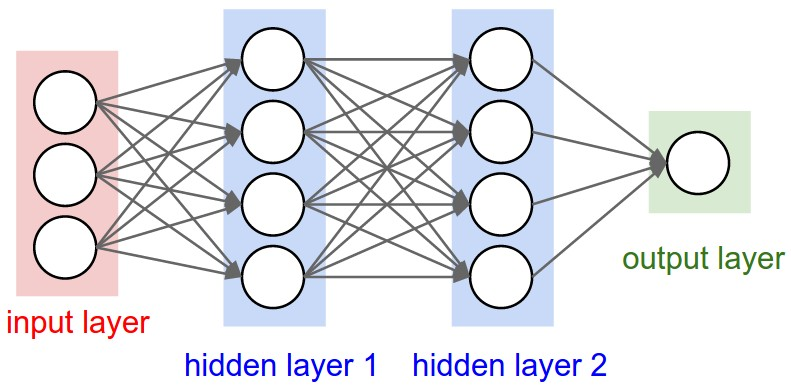
\includegraphics[width=.74\linewidth]{neural_net2.jpeg}
        \caption{Mạng neuron thông thường}\label{Fig:NN}
    \end{minipage}\hfill
        \begin {minipage}{0.48\textwidth}
        \centering
        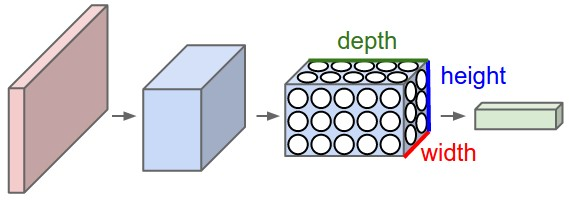
\includegraphics[width=\linewidth]{cnn.jpeg}
        \caption{Mạng tích chập neuron}\label{Fig:CNN}
    \end{minipage}
\end{figure}

Các mô hình mạng tích chập thường bắt đầu bằng một loạt các lớp tích chập kết hợp với một số lớp pooling và kết thúc bằng một (vài) lớp kết nối đặc (fully-connected).


\subsection{Lớp tích chập} 

Lớp tích chập là thành phần quan trọng nhất trong mạng tích chập neuron. Mỗi vector trọng số ở lớp này được xem như là một cửa sổ trượt, trượt trên ma trận đầu vào và thực hiện tính toán giá trị tích vô hướng tại mỗi vị trí mà cửa sổ này trượt qua. 

Các tham số quan trọng ở lớp này là \textit{kernel size}, \textit{padding} và \textit{stride}. \textit{Kernel size} là kích thước của cửa sổ trượt, được định nghĩa bằng chiều rộng ($w$), chiều cao ($h$) và chiều sâu ($d$) - chính là kích thước ma trận trọng số của lớp này. Chiều rộng và chiều cao phải nhỏ hơn hoặc bằng chiều rộng ($w^*$) và chiều cao ($h^*$) của ma trận đầu vào. \textit{Stride} ($s$) định nghĩa khoảng cách của mỗi bước trượt, trong khi \textit{padding} ($p$) quyết định xem bao nhiêu dữ liệu 0 được chèn vào rìa của ma trận đầu vào. 

Kích thước đầu ra là $W \times H \times d$ với $W = \displaystyle\frac{w^*-w+2p}{s}+1$ và $H = \displaystyle\frac{h^*-h+2p}{s}+1$. Các lớp tích chập thường sử dụng hàm kích hoạt ReLU cho vector đặc trưng ở đầu ra.

\begin{figure}[H]
    \centering
    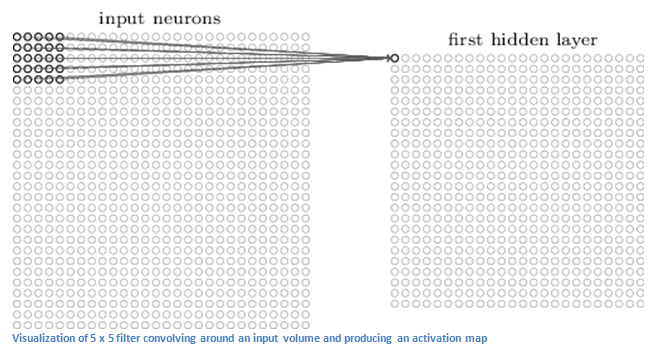
\includegraphics[width=\linewidth]{ActivationMap.png}
    \caption{Minh họa cho lớp tích chập \cite{adeshpande3cnn1}}\label{activation_map}
\end{figure}


\subsection{Lớp pooling} 

Lớp pooling thường nằm sau một lớp tích chập để làm giảm kích cỡ cũng như các dữ liệu dư thừa của vector đặc trưng. Một thuật toán pooling thường được sử dụng là max pooling. Max pooling sử dụng cửa sổ trượt trượt không trùng lắp qua ma trận đầu vào và chọn ra giá trị lớn nhất nằm trong cửa sổ để xây dựng ma trận đầu ra.

\begin{figure}[H]
    \centering
    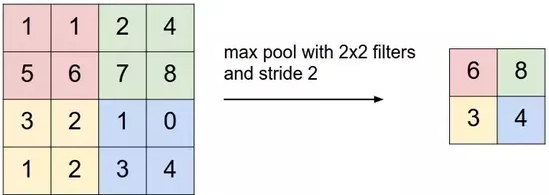
\includegraphics[width=\linewidth]{max_pooling.png}
    \caption{Max pooling}\label{max_pooling}
\end{figure}

\subsection{Lớp kết nối đặc}

Thông thường, trong các kiến trúc sử dụng mạng tích chập sẽ có các lớp kết nối đặc nằm ở cuối cùng của mô hình. Các lớp kết nối đặc phía trước có nhiệm vụ làm phẳng (flatten) vector đặc trưng trong khi lớp cuối cùng thực hiện việc dự đoán bằng một mô hình hồi quy.

\begin{figure}[H]
    \begin{minipage}{0.48\textwidth}
        \centering
        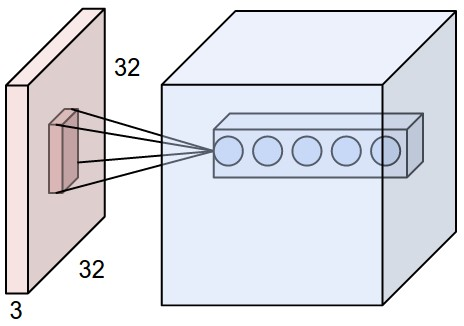
\includegraphics[width=.82\linewidth]{depthcol.jpeg}
        \caption{Một lớp convolutional}\label{Fig:depthcol}
    \end{minipage}\hfill
    \begin{minipage}{0.48\textwidth}
        \centering
        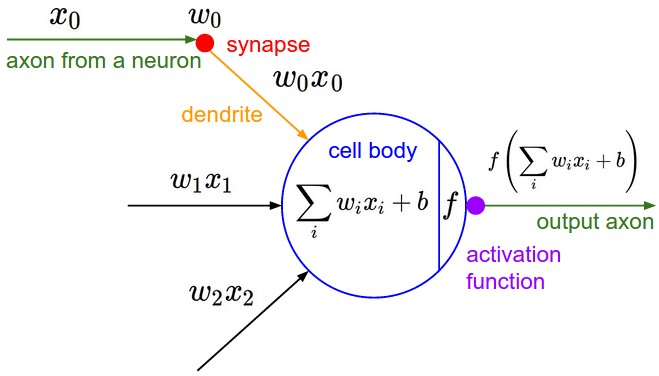
\includegraphics[width=\linewidth]{neuron_model.jpeg}
        \caption{Một neuron trong mạng}\label{Fig:neural_model}
    \end{minipage}
\end{figure}

\section{Thuật toán YOLO}

YOLO (You only look once) là một giải pháp cho bài toán nhận dạng đối tượng dựa trên mạng tích chập neuron được đề xuất bởi Joseph Redmon và các cộng sự lần đầu tiên vào năm 2015 \cite{DBLP:journals/corr/RedmonDGF15}. Không giống với các phương pháp khác, YOLO xem bài toán nhận dạng đối tượng như là một bài toán hồi quy nghĩa là vị trí của các đối tượng và lớp của chúng được tính toán bằng cách đưa giá trị các pixel của ảnh qua một mạng neuron duy nhất. YOLO có rất nhiều điểm mạnh so với các phương pháp truyền thống.

\begin{figure}[H]
    \begin{center}
        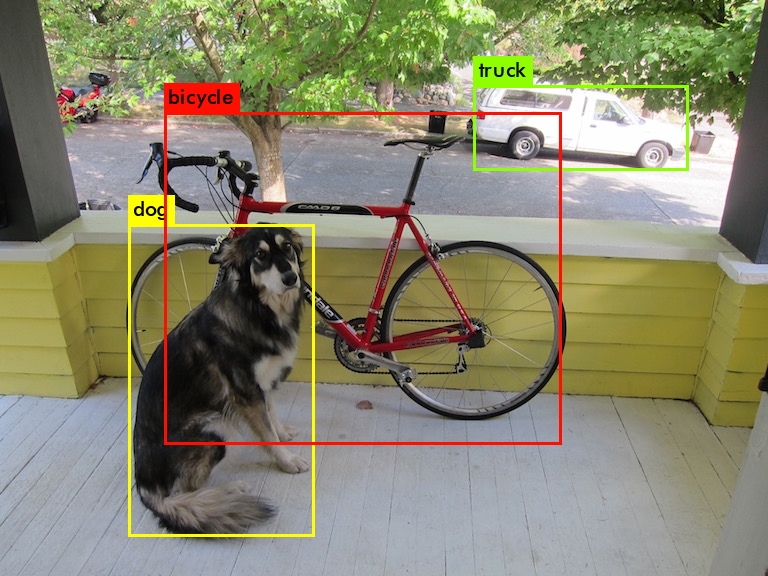
\includegraphics[width=\linewidth]{images/yolo_predictions.png}
    \end{center}
    \caption{YOLO là một giải pháp hiệu quả cho bài toán nhận dạng đối tượng}
    \label{yolo_detections}
\end{figure}

Đầu tiên, tốc độ xử lý của YOLO nhanh hơn nhiều so với các thuật toán khác trong cùng điều kiện tính toán, ảnh đầu vào trực tiếp đi qua mạng neuron mà không cần phải đi qua một ống dẫn (input pipeline) phức tạp \cite{DBLP:journals/corr/RedmonDGF15}.

Thứ hai, YOLO đánh giá sự xuất hiện của đối tượng trên toàn bộ bức ảnh, không đánh giá trên một vùng giới hạn như phương pháp cửa sổ trượt (sliding window) hay mạng RPN (region proposal network) \cite{DBLP:journals/corr/RedmonDGF15}.

\subsection{Ý tưởng của YOLO}

Ý tưởng chính của YOLO là chia ảnh đầu vào thành một lưới có kích thước là $S \times S$. Nếu điểm trung tâm của đối tượng rơi vào một ô nào đó trong lưới thì ô đó có nhiệm vụ nhận dạng đối tượng. Mỗi ô trong lưới sẽ nhận dạng $B$ khung chứa đối tượng (bounding box). Mỗi vector nhận dạng sẽ có 5 giá trị $b_x$, $b_y$, $b_w$, $b_h$ và $p$ lần lượt là hoành độ và tung độ điểm trung tâm của đối tượng trong ô đó\footnote{Tính từ điểm gốc $(0, 0)$ tại vị trí góc trên bên trái của bức ảnh}, chiều ngang và chiều cao của khung chứa đối tượng và cuối cùng là độ tin cậy. Độ tin cậy cho biết khả năng xuất hiện của đối tượng trong ô đó là bao nhiêu, nếu giá trị của $p$ thấp hơn một ngưỡng cho trước thì các giá trị còn lại không còn quan trọng.

Ngoài 5 giá trị được trình bày ở trên, vector nhận dạng còn bao gồm $C$ giá trị ($C$ bằng số lớp) biểu thị xác suất của từng lớp, giá trị $C_i$ lớn nhất nghĩa là đối tượng được nhận dạng có chỉ số bằng $i$. Vector đặc trưng của YOLO được mô tả trong hình \ref{yolo_feature_map}.

\begin{figure}[H]
    \centering
    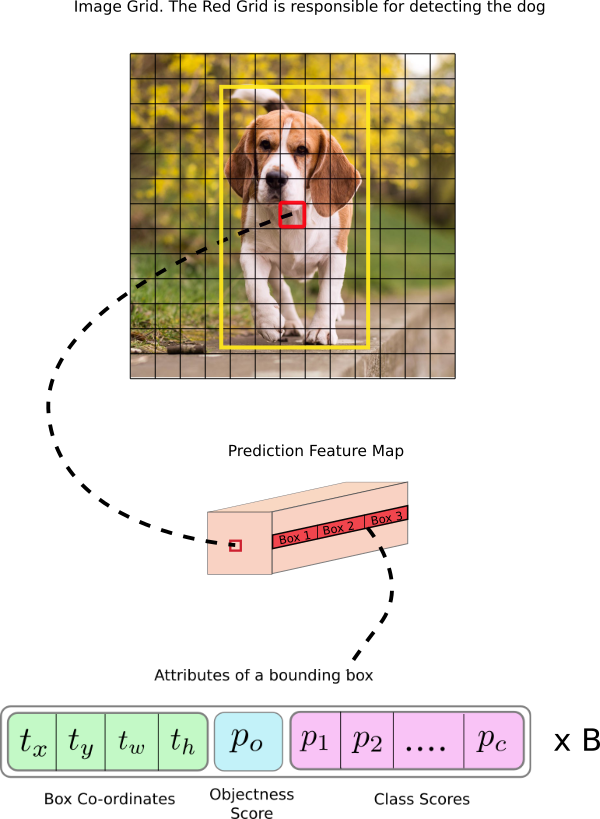
\includegraphics[width=0.9\linewidth]{images/yolo-feature-map.png}
    \caption{Cách trích xuất vector đặc trưng của YOLO \cite{yolov3-pytorch-tutorial}}
    \label{yolo_feature_map}
\end{figure}

Cần có sự phân biệt giữa $b_x$, $b_y$, $b_w$, $b_h$ và $t_x$, $t_y$, $t_w$, $t_h$. Các giá trị $t*$ là các giá trị trong vector đặc trưng, còn các giá trị $b*$ là các giá trị đã qua hàm kích hoạt, là các giá trị nhận dạng thực sự. Cụ thể với YOLOv2 và YOLOv3\footnote{Có sự khác nhau về hàm kích hoạt giữa các phiên bản YOLO.} như hình \ref{transform_feature_map}.

\begin{figure}[H]
    \centering
    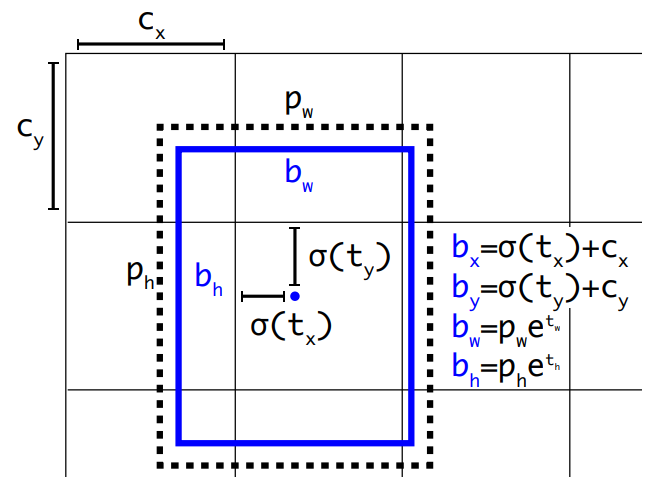
\includegraphics[width=0.5\linewidth]{images/transform_feature_map.png}
    \caption{Hàm kích hoạt của YOLOv2 và YOLOv3}
    \label{transform_feature_map}
\end{figure}

Trong đó:

\begin{itemize}[topsep=0pt]
    \item $c_x$ là \textit{offset} của ô chứa đối tượng trong lưới. Hiểu một cách đơn giản $c_x$ là chỉ số hàng của ô chứa đối tượng trong lưới\footnote{Lưu ý: chỉ số hàng và chỉ số cột tính từ 0.}.
    \item $c_y$ tương tự là chỉ số cột của ô chứa đối tượng.
    \item $a_w$ là chiều ngang của \textit{anchor box}\footnote{Khái niệm \textit{anchor box} sẽ được giải thích ở các phần sau.} có nhiệm vụ nhận dạng đối tượng.
    \item $a_h$ là chiều cao của \textit{anchor box} có nhiệm vụ nhận dạng đối tượng.
\end{itemize}

Sau quá trình nhận dạng, số lượng khung được tạo ra sẽ bằng $S\times S\times B$. 

\begin{figure}[H]
    \begin{center}
        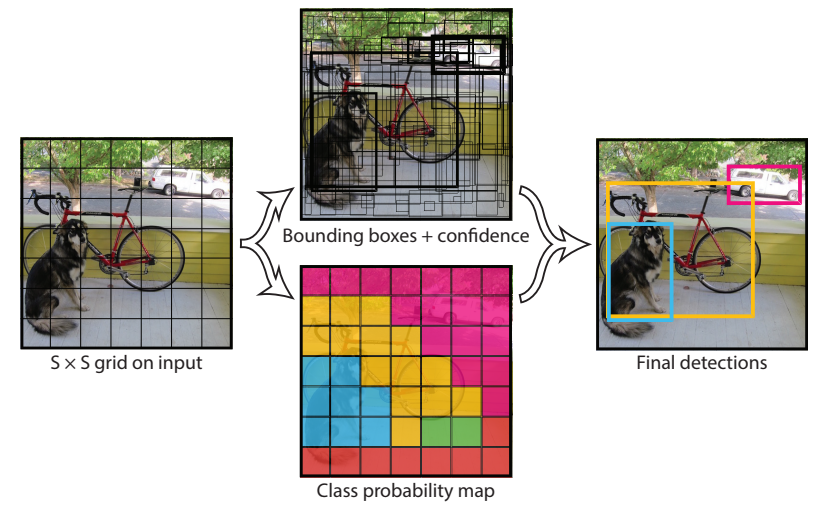
\includegraphics[width=\linewidth]{images/yolo_idea.png}
    \end{center}
    \caption{Ảnh đầu vào được chia thành lưới có kích thước là $S \times S$, mỗi ô trong lưới nhận dạng $B$ khung, mỗi khung bao gồm 4 giá trị biểu thị vị trí khung, độ tin cậy và $C$ giá trị là xác suất của mỗi lớp. Do đó mà vector nhận dạng sẽ có dạng $S \times S \times B \times (5 + C)$}
    \label{yolo_idea}
\end{figure}

Ví dụ, với tập dữ liệu \textsc{PASCAL} VOC nếu ta cho $S = 7$ và $B = 2$, tập \textsc{PASCAL} VOC có 20 lớp thì sẽ có $7 \times 7 \times 2 = 98$ khung được tạo ra và vector nhận dạng sẽ có dạng $7 \times 7 \times 2 \times 25$.

Trong số các khung được tạo ra, chỉ có một số lượng nhỏ trong số chúng là thực sự dùng để phát hiện đối tượng, để chọn ra được những khung tốt nhất, tác giả đề xuất sử dụng hai phương pháp:

\begin{itemize}[topsep=0pt]
    \item Đầu tiên, ta loại bỏ các khung có độ tin cậy nhỏ hơn một giá trị ngưỡng nào đó, mặc định trên Darknet \cite{darknet} là 0.25.
    \item Sau đó, ta sử dụng phương pháp non-max suppression để loại bỏ các khung trùng lấp lên nhau trên một đối tượng thông qua giá trị IoU.
\end{itemize} 

\subsection{Anchor box}

Trong YOLO, mỗi ô trong lưới chỉ nhận dạng duy nhất một đối tượng, giả sử rằng điểm trung tâm của hai đối tượng cùng rơi vào một ô thì ô đó sẽ nhận dạng đối tượng nào? Chắc chắn sẽ có một đối tượng bị bỏ qua. Để giải quyết vấn đề đó, YOLO sử dụng các \textit{anchor box}. Tại mỗi ô trong lưới, thay vì chỉ nhận dạng một khung chứa đối tượng duy nhất thì ta sẽ sử dụng $B$ khung chứa đối tượng khác nhau, chúng có kích thước cũng như tỉ lệ khác nhau giúp cho việc nhận dạng được tốt hơn. 

\begin{figure}[H]
    \begin{center}
        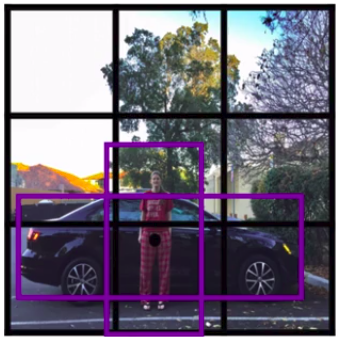
\includegraphics[width=0.5\linewidth]{images/anchor_box.png}
    \end{center}
    \caption{Sử dụng 2 anchor boxes cho một ô \cite{cnn-ang}}
    \label{anchor_box}
\end{figure}

Dễ dàng nhận thấy trên hình \ref{anchor_box}, điểm trung tâm của khung chứa chiếc ô tô và khung chứa người (chấm tròn màu đen) cùng rơi vào một ô. Tuy nhiên, hình người là một hình chữ nhật thẳng đứng, còn xe ô tô lại là một vật thể nằm ngang, sử dụng 2 anchor boxes có kích thước khác nhau như vậy sẽ giúp nhận dạng được các đối tượng một cách tốt hơn. 

Việc sử dụng anchor box có hai tác dụng:

\begin{itemize}[topsep=0pt]
    \item Giải quyết được đa phần các trường hợp có nhiều đối tượng rơi vào cùng một ô.
    \item Giúp cho kết quả nhận dạng tốt hơn do kích thước và hình dạng của các đối tượng khác nhau, việc sử dụng nhiều hơn một anchor box sẽ giúp ta bắt được nhiều trường hợp hơn.
\end{itemize}

\subsection{Chỉ số IoU}

Intersection over Union (IoU) là tỉ số giữa phần giao nhau giữa hai tập hợp và phần kết hợp giữa chúng. Trong bài toán nhận dạng đối tượng, IoU giữa hai khung chứa đối tượng là tỉ số giữa diện tích phần chung của hai khung và tổng diện tích phần kết hợp giữa hai khung đó.

\begin{figure}[H]
    \begin{center}
        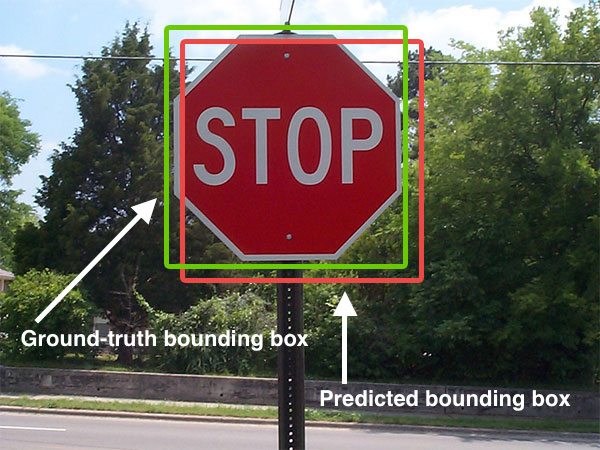
\includegraphics[width=0.7\linewidth]{images/traffic_sign_iou.jpg}
    \end{center}
    \caption{Khung chứa đối tượng thực tế và khung được dự đoán \cite{jaccard_index}}
    \label{traffic_sign_iou}
\end{figure}

Công thức tính giá trị IoU giữa hai khung chứa đối tượng như hình \ref{iou_equation}.

\begin{figure}[H]
    \begin{center}
        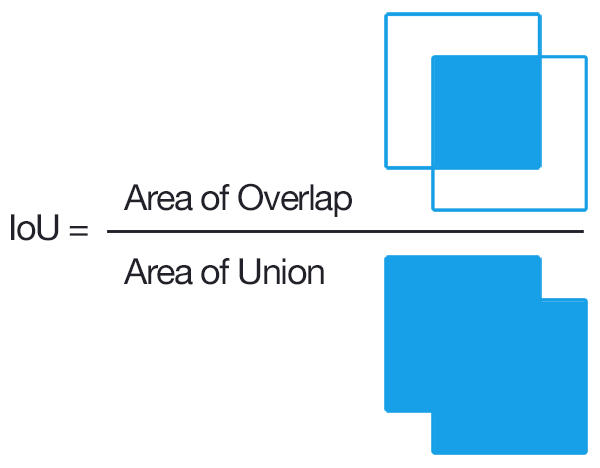
\includegraphics[width=0.55\linewidth]{images/Intersection_over_Union_-_visual_equation.png}
    \end{center}
    \caption{Công thức tính giá trị IoU \cite{jaccard_index}}
    \label{iou_equation}
\end{figure}

\subsection{Non-max suppression}

Non-max suppression là một phương pháp loại bỏ các khung trùng nhau trên một đối tượng. Giả sử $L$ là một danh sách các khung thuộc cùng một lớp. Mã giả của non-max suppression được trình bày như sau:

\begin{Verbatim}
sort_descending(L);
forall i in {0..(size(L) - 2)} do
    forall j in {i+1..(size(L) - 1)} do
        if IoU(L[i], L[j]) >= 0.5 then
            drop L[j];
\end{Verbatim}

Sau quá trình thực hiện non-max suppression, các khung còn lại trong $L$ là các khung chứa đối tượng được dự đoán bởi YOLO.

\subsection{Hàm mất mát}

Hàm mất mát (loss function) của YOLO là một hàm mất mát nhiều thành phần:

\begin{itemize}
    \begin{item}
        Hàm mất mát tại các ô không có đối tượng xuất hiện:
        \begin{align*}
            L_1 = \lambda_\text{noobj}\displaystyle\sum_{i=0}^{S^2}\sum_{j=0}^{B}{\mathbbm{1}^\text{noobj}_{ij}\left(p_i-\hat{p_i}\right)^2}
        \end{align*}
        Trong đó $\mathbbm{1}^\text{noobj}_{ij}$ ký hiệu cho việc không có đối tượng xuất hiện trong ô thứ $i$ và anchor box thứ $j$, $\hat{p_i}$ là độ tin cậy được dự đoán bởi mô hình và $p_i$ là độ tin cậy thực tế.
    \end{item}
    
    \begin{item}
        Hàm mất mát tại các ô có đối tượng xuất hiện:
        \begin{align*}
            L_2 = \displaystyle\sum_{i=0}^{S^2}\sum_{j=0}^{B}{\mathbbm{1}^\text{obj}_{ij}\left(p_i-\hat{p_i}\right)^2}
        \end{align*}
        Trong đó $\mathbbm{1}^\text{obj}_{ij}$ ký hiệu cho việc có đối tượng xuất hiện trong ô thứ $i$ mà cụ thể là ở anchor box thứ $j$.
    \end{item}
  
    \begin{item}
        Hàm mất mát cho bài toán phân lớp:
        \begin{align*}
            L_3 = \displaystyle\sum_{i=0}^{S^2}{\mathbbm{1}^\text{obj}_i}\sum_{c \in \text{classes}}{\left(c_i(c) - \hat{c_i}(c)\right)^2}
        \end{align*}
        Trong đó $\mathbbm{1}^\text{obj}_{i}$ ký hiệu cho việc có đối tượng xuất hiện trong ô thứ $i$, $c_i(c)$ và $\hat{c_i}(c)$ lần lượt là xác suất của lớp $c$ trong ô thứ $i$ trong thực tế cũng như là được dự đoán bởi mô hình.
    \end{item}

    \begin{item}
    Hàm mất mát cho bài toán hồi quy tìm vị trí của đối tượng trong ảnh:
    \begin{align*}
        L_4 &= \lambda_\text{coord}\displaystyle\sum_{i=0}^{S^2}\sum_{j=0}^{B}{\mathbbm{1}^\text{obj}_{ij}\left[(x_i - \hat{x}_i)^2 + (y_i - \hat{y}_i)^2\right]}\\
        &\quad + \lambda_\text{coord}\displaystyle\sum_{i=0}^{S^2}\sum_{j=0}^{B}{\mathbbm{1}^\text{obj}_{ij}}\left[\left(\sqrt{w_i} - \sqrt{\hat{w}_i}\right)^2 + \left(\sqrt{h_i} - \sqrt{\hat{h}_i}\right)^2\right]
    \end{align*}
    \end{item}
\end{itemize}

Kết hợp các hàm mất mát thành phần trên, ta được hàm mất mát của YOLO là:

\begin{align*}
    L = L_1 + L_2 + L_3 + L_4
\end{align*}

Trong hàm mất mát của YOLO có sử dụng 2 tham số là $\lambda_\text{coord}$ và $\lambda_\text{noobj}$ nhằm cân chỉnh giá trị của hàm mất mát, tăng giá trị hàm mất mát tại các neuron nhận dạng vị trí của đối tượng và giảm tại các neuron dự đoán độ tin cậy. Giá trị của các tham số này là: $\lambda_\text{coord} = 5$ và $\lambda_\text{noobj} = 0.5$.

\subsection{Các phiên bản của YOLO}

\subsubsection{Phiên bản 1 (YOLOv1)}

Phiên bản đầu tiên của YOLO sử dụng 24 lớp tích chập cho việc trích lọc đặc trưng và 2 lớp kết nối đặc cho việc nhận dạng đối tượng. Kiến trúc của YOLOv1 như hình \ref{yolov1}.

\begin{figure}[H]
    \centering
    \includegraphics[width=\linewidth]{net}
    \caption{Kiến trúc của YOLOv1}
    \label{yolov1}
\end{figure}
   
\subsubsection{Phiên bản 2 (YOLOv2)}

YOLOv2 là phiên bản cải tiến của YOLOv1 cả về độ chính xác cũng như thời gian nhận dạng. 

YOLOv2 sử dụng phương pháp \textit{batch normalization} trên các lớp tích chập thay vì sử dụng các lớp \textit{dropout} sau các lớp kết nối đặc, điều này đã giúp tăng mAP lên 2\%.

Với YOLOv1, kích thước của các \textit{anchor box} được lựa chọn một cách ngẫu nhiên, với cách làm này, thuật toán sẽ hoạt động hiệu quả với một số loại đối tượng nhưng lại ảnh hưởng đến các đối tượng khác. Từ phiên bản 2 của YOLO, tác giả đề xuất sử dụng thuật toán \textit{k-means}, cụ thể là duyệt qua toàn bộ tập dữ liệu để phân cụm kích thước các khung chứa đối tượng, từ đó đề xuất giá trị của các \textit{anchor box} sao cho phù hợp hơn.

Thay vì sử dụng 2 lớp kết nối đặc (fully-connected) ở cuối mạng neuron, YOLOv2 bỏ qua các lớp này và tiến hành nhận dạng trên vector đặc trưng từ các lớp tích chập phía trước theo một cách khác như hình \ref{transform_feature_map}.

\subsubsection{Phiên bản 3 (YOLOv3)}
  
YOLOv3 có nhiều cải tiến so với các phiên bản trước, đặc biệt là chiến lược sử dụng nhiều kích thước khác nhau của lưới nhận dạng (multi-scales). Thay vì chỉ sử dụng một lưới có kích thước cố định là $S \times S$ như các phiên bản trước thì YOLOv3 sử dụng 3 lưới có kích thước lần lượt là $13 \times 13$, $26 \times 26$, $52 \times 52$ sau đó kết hợp các kết quả nhận dạng lại trước khi áp dụng ngưỡng và non-max suppression, cách làm này khiến cho YOLOv3 có khả năng nhận dạng các vật thể nhỏ tốt hơn và tăng độ chính xác. 
  
\end{document}
